\documentclass[11pt]{article}
\usepackage[utf8]{inputenc}
\usepackage[bulgarian]{babel}
\usepackage{geometry}
\geometry{a4paper}
\usepackage{graphicx}
\graphicspath{ {.} }
\usepackage{booktabs}
\usepackage{array}
\usepackage{paralist}
\usepackage{verbatim}
\usepackage{subfig}
\usepackage{fancyhdr}
\pagestyle{fancy}


\renewcommand{\headrulewidth}{0pt}
\lhead{}\chead{}\rhead{}
\lfoot{}\cfoot{\thepage}\rfoot{}

\usepackage{sectsty}

\allsectionsfont{\sffamily\mdseries\upshape}

\usepackage[nottoc,notlof,notlot]{tocbibind} 
\usepackage[titles,subfigure]{tocloft} 
\renewcommand{\cftsecfont}{\rmfamily\mdseries\upshape}
\renewcommand{\cftsecpagefont}{\rmfamily\mdseries\upshape}

\usepackage{physics}
\usepackage{amsmath}
\usepackage{centernot}
\usepackage{url}
\usepackage{enumitem}

\title{4. Контекстно-свободни граматики. Стекови автомати}
\begin{document}
\maketitle

\newcommand{\lrangle}[1]{\left\langle #1 \right\rangle}

\newcommand{\belongsTo}{\in}
\newcommand{\notBelongsTo}{\centernot\in}

\newcommand{\oversetModels}[1]{\overset{#1}{\models}}

\newcommand{\kda}{A = <Q, X, q_{0}, \delta, F>}
\newcommand{\cfg}{\Gamma = <\mathcal{N}, \mathcal{T}, \mathcal{S}, \mathcal{P}>}
\newcommand{\cfgVers}{G = \langle V, \Sigma, R, S \rangle}
\newcommand{\nsa}{A = <Q, X, Z, q_{0}, z_{0}, \delta, F>}

\newcommand{\italicBold}[1]{\textbf{\emph{#1}}}
\newcommand{\definition}{\italicBold{Дефиниция: }}
\newcommand{\theorem}{\italicBold{Теорема: }}
\newcommand{\lemma}{\italicBold{Лема: }}
\newcommand{\proof}{\italicBold{Доказателство: }}
\newcommand{\sample}{\italicBold{Пример: }}

\newcommand{\curlies}[1]{\{#1\}}

\newcommand{\enumNum}{\renewcommand{\theenumi}{\arabic{enumi}}}
\newcommand{\enumlet}{\renewcommand{\theenumi}{\alph{enumi}}}

\italicBold{Анотация:} Контекстно-свободни граматики. Дървета за синтактичен анализ. Нормална форма на Чомски. Стекови автомат. Връзка между стековите автомати и контекстно-свободните граматики (доказателство в една посока по избор). Свойства на затвореност. Лема за покачването (xyuvw)(с доказателство). Примери за езици, които не са контекстно-свободни.

\section{Контекстно-свободни граматики}

\definition \textbf{Контекстно-свободна граматика}: КСГ наричаме четворката $G = (V, \Sigma, R, S)$, където
\begin{itemize}[noitemsep]
	\item $V$ е крайно множество от \textit{променливи}
	\item $\Sigma$ е крайно множество от \textit{букви}, $\Sigma\cap V = \emptyset$. $\Sigma$ наричаме още множество от терминали.
	\item $R \subseteq V \times (V \cap \Sigma)^{*}$, крайно множество от \textit{правила}
	\item $S \in V$ е началната променлива
\end{itemize}

При дадена граматика $G$ за правилата на граматиката обикновено ще пишем $A \to \alpha$ вместо $(A, \alpha) \in R$. Ще въведем релация между думи $\alpha, \beta \in (V \cup \Sigma)^{*}$, която ще казва, че думата $\beta$ се получава от $\alpha$ като приложим правило от граматиката. За две думи $u, v \in (V \cup \Sigma)^{*}$ ще пишем $u \to_{G}\;v$, ако съществуват думи $x, y \in (\Sigma \cup V)^{*}, A \in V$, правило $A \to \alpha$ и $u = xAy, v = x \alpha y$. С $\to^{*}_{G}$ ще означаваме рефлексивното и транзитивно затваряне на релацията $\to_{G}$.

Езикът породен от граматиката $G$ е множеството от думи $\mathcal{L}(G)=\curlies{\alpha \in \Sigma^{*} | S \to^{*}_{G}\alpha}$.\\

Всяка последователност от вида $w\textsubscript{0}\to_{G}w\textsubscript{1}\to_{G}w\textsubscript{2}\to_{G}... w\textsubscript{n}$ наричаме \textit{извод} в  $G$ от $w\textsubscript{0}$ до $w\textsubscript{n}$. Тук $w\textsubscript{0}, ..., w\textsubscript{n}$ са произволни думи от $V^*$, а $n$ наричаме \textit{дължина} на извода, $n\in N$. Казваме още, че изводът има $n$ стъпки. \\

\sample Следната граматика генерира всички изрази с правилно вложени скоби - всяка лява скоба трябва да има съответстваща дясна, и всяка затваряща трябва да има уникална съответстваща отваряща скоба. Нещо повече, низовете между всяка такава двойка скоби трябва да отговарят на същото условие. Нека $\Gamma = < V, \Sigma, R, S>$, където: $V = \curlies{{ s, (, )}}, \Sigma = \curlies{{(,)}}, R = \curlies{ {s\to\epsilon, s\to ss, s\to(s)}}$. Два извода от тази граматика са:
$s \to ss \to s(s) \to s((s)) \to s(()) \to ()(())$ и $s \to ss \to (s)s \to ()s \to ()(s) \to ()(())$.
Следователно една дума може да има няколко различни извода в една граматика. $L(G)$ е пример за език, който е контекстно-свободен. но не е регулярен.\\
Очевидно има примери за езици, които са контекстно-свободни, но не са регулярни. 

\section{Дърво на синтактичен анализ}
Нека $G$ е КСГ. Както показахме думата $w \in L(G)$ може да има много изводи в G. Например в разгледаната по-горе граматика за правилно вложени скоби, думата ()() може да получена от $S$ чрез поне два различни извода: $S \to SS \to (S)S \to ()S \to ()()$ и $S \to SS \to S(S) \to (S)(S) \to (S)() \to ()()$. Ако разгледаме внимателно тези два извода, ще забележим, че са еднакви - различават се единствено по реда на прилагане на правилата. Интуитивно и двете могат да бъдат означени графично така:\\
\centerline{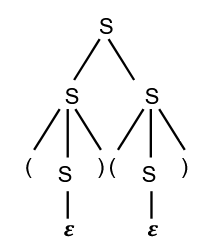
\includegraphics[scale=0.5]{imgDTree.png}}\\
Диаграма от горния тип наричаме дърво на синтактичен анализ. Символите наричаме върхове, като всеки връх е означен със символ от V. Най-горният връх се нарича корен, а най-долните листа. Всички листа са означени или с терминални символи или с празната дума $\epsilon$. Ако "проследим" листата на дървото, ще получим дума, която се нарича резултат на дървото на синтактичния анализ.\\
Или казано по-формално - на всеки извод в контекстно-свободната граматика ще  съпоставим дървовидна структура със следната дефиниция:\\
\definition Нека $\cfg$ е контекстно-свободна граматика. Дървото $D(V, E)$ с корен $r \in V$, с наредба на синовете и функция $f: V \to (N \cup T)$ <съпоставяща на всеки връх буква от азбуките на граматиката, наричаме \emph{дърво на синтактичен анализ} в $\Gamma$, ако 

\enumlet
\begin{enumerate}
	\item За всеки нелист $v$ на $D, f(v) \in N$, като $f(r) = S$;
	\item За всеки лист $l$ на $D, f(l) \in T$;
	\item За всеки нелист $v$ с наредена последователност от синове $v_{i_1}, v_{i_2}, ..., v_{i_k}$, е в сила $f(v_{i_1})f(v_{i_2})...f(v_{i_k})\in P$. 
\end{enumerate}

\definition Нека $D(V, E)$ е дърво на синтактичен анализ в граматиката $\cfg$

\enumlet
\begin{enumerate}
	\item Ако $D$ е дърво от вида $S$-------$\epsilon$, то дума на $D$ е $\epsilon$;
	\item Нека $D'(\curlies{l}, \curlies{})$ е поддърво на дървото на извод $D$, състоящо се само от лист $l$. Дума на $D'$ е $f(l)$;
	\item Нека $D'$ е поддърво на $D$ с корен $r', D_{1}, D_{2}, ..., D_{k}$ са всички поддървета на $D'$ с корени синовете на $r'$, подредени в съответствие с наредбата на тези синове и $\alpha_{i}$ е думата на поддървото $D_{i}, i = 1, 2, ..., k$. Тогава думата на $D'$ е $\alpha_{1}, \alpha_{2}, ...,\alpha_{k}$. 
\end{enumerate} \par

\theorem Нека $\cfg$ е КСГ. Съществува дърво на извод (синтактичен анализ) $D$ в $\Gamma_{A}$ с дума $\omega$, за което $A^{\Gamma} \models^{A} \omega$ \\


\definition Ако в КСГ $\Gamma$ съществува повече от едно дърво на извод (дърво за синтактичен анализ) за някоя дума $\omega$, тогава наричаме $\Gamma$ \emph{еднозначна}. \\ 

\definition КСЕ (контекстно-свободен език) $L$, за който всяка КСГ, която го поражда е нееднозначна, наричаме \emph{нееднозначен език}. 

\section{Нормална форма на Чомски}
\definition Една КСГ е в нормална форма на Чомски, ако всяко правило е от вида $A \to BC$ и $A \to \alpha$. Като $B$ и $C$ не могат да бъдат променливата за начало $S$. Освен това позволяваме правилото $S \to \epsilon$

\theorem За всяка КСГ $G$ съществува КСГ $G'$ в Нормална форма на Чомски, такава, че $L(G') = L(G) - (\Sigma \cup \curlies{{\epsilon}})$

\section{Стекови автомати}
\subsection{Недетерминирани стекови автомати}
Не всеки контекстно-свободен език може да бъде разпознат от крааен автомат, понеже не всеки контекстно-свободен език е регулярен. Затова трябва да дефиниране по-сложни машини, разпознаващи тези езици. Важното за тези езици е понятието \emph{стек}. Стекът е запомнящо устройство, в което могат да се записват буквите на някаква азбука $Z$, и да се вземат обратно от стека, когато е необходимо. Това означава, че всеки новозапомнен елемент се поставя над елемента, обозначен като връх на стека и сам става връх. Когато трябва да се вземе елемент от стека, това непременно е върхът и връх става елементът, който е влязъл непосредствено преди него. Освен тези две операции, понякога се ползва и операцията четене от стека, което означава, че се прочита буквата на върха, без да се изважда от стека. \par

Абстрактната машина, която ще опишем, разполага с обичаен вход, от който може да четат буквите на входна азбука $X$ и стек, от който може да чете и в който може да пише. Машината може да се намира в крайно множество от състояния. \\

\definition Недетерминиран стеков автомат наричаме седморката \\$\nsa$, в която: $Q$ е крайно множество от състояния; $X$ е крайна входна азбука; $Z$ е крайна стекова азбука; $q_{0} \in Z$ е начална стекова буква; $\delta: Q \times (X \cup \curlies{\epsilon}) \times Z \to 2^{Q \times Z^*}$ е частична функция на преходите; $F \subseteq Q$ е множество от заключителни състояния. \par

\begin{itemize}
	\item Специалната буква $z_{0}$ в стековата азбука е предназначена да пази стека от презаписване, тъй като НСА не може да работи без да чете букви от стека. Противно на КДА четенето на входна буква от $X$ не е задължително за НСА (забележете, че $X \cup \curlies{\epsilon}$ е в дефиниционната област на $\delta$). С други думи НСА може да работи без да чете входни данни, обработвайки запомнената в стека дума.
	\item Втората особеност е по-сложната функция на преходите $\delta$, дефинирана върху тройки (състояние, входна буква или празна дума, стекова буква). В резултата на всяка стъпка на НСА може да премине недетерминирано в някое от определените от $\delta$ състояния, замествайки буквата във във върха на стека със съответната, зададена от $\delta$, дума.  
\end{itemize} 

За формално дефиниране на работата на НСА, да определим неговото текущо положение с тройката $<q, \alpha, \gamma>$, наречена \emph{конфигурация} на НСА, в която $q$ е текущото състояние на автомата, а $\gamma$ текущата стекова дума, четена от върха към дъното на стека. Очевидно, конфигурацията точно определя текущото положение на НСА и бъдещето му поведение. \\

\definition Релацията $R_{\models} \subseteq K_{A} \times K_{A}$ дефинираме като рефлексивно и транзитивно затваряне на $R_{\vdash}$. Ако $k_{1}, k_{2} \in K_{A}$ и $k_{1} \models k_{2}$ казваме, че конфигурацията на $k_{1}$ може да се трансформира в $k_{2}$. \par

\definition НСА $\nsa$ \emph{разпознава със заключително състояние} думата $\alpha$, ако съществува $q \in F$, такова че $< q_{0},\alpha, z_{0}> \models < q, \epsilon, \gamma >$, независимо от това каква е $\gamma$. Езикът $L_{A}^{F} = \curlies{\alpha | \exists q \in F, < q_{0}, \alpha, z_{0} > \models < q, \epsilon, \gamma>}$, наричаме език, разпознавам със заключителни състояния от НСА $A$. \par

\definition Казваме че НСА $A = < Q, X, Z, q_{0}, z_{0}, \delta, \emptyset>$ \emph{разпознава с празен стек} думата $\alpha$, ако $< q_{0}, \alpha, z_{0} > \models < q, \epsilon, \epsilon>$, независимо от това какво е състоянието $q$. Езикът $L_{A}^{\emptyset} = \curlies{\alpha | < q_{0}, \alpha, z_{0}> \models < q, \epsilon, \epsilon>}$, наричаме език, разпознат с празен стек от НСА $A$. 

\subsection{Връзка между НСА и КСГ}
\theorem За всеки НСА $A$, разпознаващ езика $L$ съществува КСГ $\Gamma$ такава, че $L = L_{G}$.\\
\proof Ще разгледаме двете посоки на твърдението поотделно.

\enumNum
\begin{enumerate}
	\item Нека е дадена безконтекстна граматика $\cfgVers$. Нашата цел е да построим стеков автомат $P$, така че $L_{s}(P) = L(G)$. Нека $P = \langle \curlies{q}, \Sigma, \Sigma \cup V, S, q, \Delta, \emptyset$,	където функцията на преходите е: $\Delta(q, \epsilon, A) = \curlies{(q, \alpha) | A \to \alpha е правило в граматиката G}$, $\Delta(q, \alpha, \alpha) = \curlies{(q, \epsilon)}$
	\item Нека имаме $P = \langle Q, \Sigma, \Gamma, \Delta, s, \#, \emptyset \rangle$. 
	Ще дефинираме безконтекстна граматика $G$, за която $L_{S}(P) = L(G)$. Променливите на граматиката са $V = \curlies{[q, A, p] | q, p \in Q, A \in \Gamma}$.
\end{enumerate}
Правилата на $G$ са следните:
\begin{itemize}
	\item $S \to [s, \#, q]$, за всяко $q \in Q$; 
	\item $[q, A, q_{m+1}] \to a[q_{1}, B_{1}, q_{2}][q_{2}, B_{2}, q_{3}]...[q_{m}, B_{m}, q_{m+1}]$, където $(q_{1}, B_{1}...B_{m}) \in \Delta(q, a, A)$ и произволни $q, q_{1}, ..., q_{m+1} \in Q, a \in \Sigma \cup \curlies{\epsilon}$. Да обърнем внимание, че е възможно $m = 0$. Това означава, че $(q_{1}, \epsilon) \in \Delta(q, a, A)$ и тогава имаме правилото $[q, A, q_{1}] \to a$, където $а \iн \Sigma \cup \curlies{\epsilon}$. \\
	Трябва да докажем, че: $[q, A, p]\to^{*}_{G} \alpha \leftrightarrow (q, \alpha, A) \vdash^{*}_{P}(p, \epsilon, \epsilon)$.
\end{itemize}
$(\rightarrow)$ С пълна индукция по $i$ ще докажем, че $(q, \alpha, A) \vdash^{i}_{P} (p, \epsilon, \epsilon) \rightarrow [q, A, p] \rightarrow^{*}_{G} \alpha$.\\

Ако $i = 1$, то е лесно, защото $\alpha \in \Sigma \cup \curlies{\epsilon}$ и $m = 0$.\\

Ако $i > 1$, нека $\alpha = a \beta$. Тогава: $(q, a \beta,A)\vdash_{P}(q_{1}, \beta, B_{1}...B_{n})\vdash^{i-1}_{P}(p, \epsilon, \epsilon)$.\\

Да разбием думата $\beta$ на $n$ части, $\beta = \beta_{1}...\beta_{n}$, със свойството, че след като прочетем $\beta_{i}$ сме премахнали променливата $B_{i}$ от върха на стека. Това означава, че: \\
\centerline{$(q_{j}, \beta_{j}, B_{j}) \vdash^{l_j}_{P}(q_{j+1, \epsilon, \epsilon})$, за $j = 1, ..., n-1$,}\\
\centerline{$(q_{n}, \beta_{n}, B_{n}) \vdash^{l_n}_{P}(p, \epsilon, \epsilon)$,}\\
където $l_{1} + l_{2} + ... + l_{n} = i - 1$. Сега по \textbf{ИП} получаваме:\\
$(q_{j}, \beta_{j}, B_{j})\vdash^{l_j}_{P}(q_{j+1}, \epsilon, \epsilon) \rightarrow [q_{j}, B_{j}, q_{j+1}] \to^{*}_{G}\beta_{j}$, за $j = 1, ..., n - 1$, \\
$(q_{n}, \beta_{n}, B_{n})\vdash^{l_n}_{P}(p, \epsilon, \epsilon) \rightarrow [q_{n}, B_{n},p] \to^{*}_{G}\beta_{n}$.\\
Обединявайки тези изводи с правилото $[q, A, p] \to_{G} a[q_{1}, B_{1}, q_{2}]...[q_{n}, B_{n}, p]$, получавам извода $[q, A, p] \to ^{*}_{G} a \beta$\\ 

($\leftarrow$) Отново с пълна индукция по $i$ ще докажем, че $[q, A,p] \to^{i}_{G}\alpha \rightarrow (q, \alpha, A) \vdash^{*}_{P} (p, \epsilon, \epsilon) $.\\

Ако $i = 1$, то имаме $[q, A, p] \to \alpha$, където $\alpha = a$ или $\alpha = \epsilon$. Ако $i > 1$, то имаме, че $\alpha = a \beta$ и за някое $n$, $[q, A, p] \to_{G} a[q_{1}, B_{1}, q_{2}][q_{2}, B_{2}, q_{3}]...[q_{n}, B_{n}, p] \to^{i-1}_{G} \beta$.\\

Отново нека $\beta = \beta_{1}...\beta_{n}$, където $[q_{j}, B_{j}, q_{j+1}] \to ^{i_j}_{G} \beta_{j}$, за $j = 1, ..., n-1$,\\
$[q_{n}, B_{n}, p] \to ^{i_n}_{G} \beta_{n}$, където $i_{1} + i_{2} + ... + i_{n} = i - 1$. От \textbf{ИП} получаваме, че \\
\centerline{$[q_{j}, B_{j}, q_{j+1}] \to ^{i_j}_{G} \beta_{j} \rightarrow (q_{j}, \beta_{j}, B_{j}) \vdash^{*}_{P}(q_{j+1}, \epsilon, \epsilon), j = 1, ..., n - 1$}\\
\centerline{$[q_{n}, B_{n}, p] \to ^{i_n}_{G}\beta_{n} \rightarrow (q_{n}, \beta_{n}, B_{n}) \vdash^{*}_{P}(p, \epsilon, \epsilon)$.}\\

Обединяквайки всичко което знаем, получаваме: \\
\centerline{$(q, a \beta, A)\vdash_{P}(q_{1}, \beta_{1}...\beta_{n}, B_{1}...B_{n})$}\\
\centerline{$\vdash^{*}_{P}(q_{2}, \beta_{2}...\beta_{n}, B_{2}...B_{n})$}\\
\centerline{...}\\
\centerline{$\vdash^{*}_{P}(q_{n}, \beta_{n}, B_{n})$}\\
\centerline{$\vdash^{*}_{P}(p, \epsilon, \epsilon)$}\par

\section{Свойства на затвореност}
\begin{itemize}
	\item Обединение: Ако $L_{1}$ и $L_{2}$ са два КСЕ, тяхното обединение $L_{1} \cup L_{2}$ също е контекстно-свободно. $\rightarrow$ КСЕ са затворени под операцията Обединение. 
	\item Конкатениране:  Ако $L_{1}$ и $L_{2}$ са два КСЕ, тяхната конкатенация $L_{1}.L_{2}$ също е контекстно-свободна. $\rightarrow$ КСЕ са затворени под операцията Конкатенация. 
	\item Звезда на Клини: Ако $L_{1}$ е контекстно-свободен, то $L_{1}^{*}$ също е контекстно-свободен. $\rightarrow$ КСЕ са затворени под операцията Звезда на Клини. 
	\item Сечение и Множествена разлика: Ако $L_{1}$ и $L_{2}$ са два КСЕ, тяхното сечение $L_{1} \cap L_{2}$ \textbf{не} е задължително контекстно-свободно. $\rightarrow$ КСЕ \textbf{не} са затворени под операцията Сечение и Множествена разлика ($A \setminus B$) . 
	\item Детерминистични КСЕ: Те са подмножество на КСЕ, които могат да бъдат разпознати от КДА. Те са затворени единствено под операциите Множествена разлика и Обратен хомоморфизъм.  
\end{itemize}

\section{Лема за покачването (xyuvw)}
\lemma \italicBold{Лема за покачването:} За всеки непразен КСЕ $L \neq \curlies{\epsilon}$ съществува цяло $n > 0$ такова, че ако $\alpha \in L, d(\alpha) > n$, то $\alpha = xyuvw$ и:

\enumNum
\begin{enumerate}
	\item $d(u) \geq 1, d(yv) \geq 1, d(yuv) \leq n$;
	\item $xy^{i}uv^{i}w \in L, \forall i = 0, 1, 2, ...$
\end{enumerate}
\proof Нека $\cfg$ е КСГ без преименуващи правила, която поражда езика $L$. Нека $l = |\mathcal{N}|$, а $m = \underset{\forall A \to \beta \in \mathcal{P}}{max} d(\beta), m \geq 1$. Нека $n = m^{l + 1}$. Ще покажем, че това е търсеното цяло положително число. Нека $\alpha \in L, d(\alpha) > n$. Нека $D$ е дърво на извод за $\alpha$ в $\Gamma$ с височина $h$. Тъй като $D$ е дърво на извод, всеки връх има $\leq m$ сина и съгласно \\
 
\theorem Нека $D(V, E)$ е кореново дърво и реброто $(v_{i}, v_{j}) \notin E$. Тогава графът $G(V, E \cup \curlies{(v_{i}, v_{j})})$  съдържа единствен цикъл \\

броят на листата му е $d(\alpha) \leq m^{h}$. Следователно $m^{l+1} = n < d(\alpha) \leq m^{h}$ или $m^{l+1} < m^{h}$. От монотонността на показателната функция при $m \geq 1$ получаваме, че $l + 1 < h$. Но височината на $D$ е равна на броя на нетерминалите , последователно срещащи се по най-дългия път от корена до някой лист (последния връх на пътя е означен с терминал). Следователно този брой е $> l$. От принципа на Дирихле следва, че по този път поне един нетерминал $A$ ще се срещне поне два пъти. Да изберем най-близките до листа две срещания на $A$ (такива, че след по-близкото до корена срещане няма друг нетерминал, който се среща поне два пъти). 

С $D'(V', E')$ означаваме поддървото с корен по-близкия до корена на $D$ нетерминал $A$, а с $D''(V'', E'')$ поддървото с корен по-далечният от корена на $D$ нетерминал $A$. Сега думата $\alpha$ на $D$ естествено се разпада на пет поддуми $x, y, u, v, w$ така, че $u$ е думата на поддървото $D''$(в граматиката $\Gamma_{A}$), $y$ - поддумата от листата на $D'$ и на $D'', x$ - поддумата от листата на $D$, стоящи вляво от листата на $D'$ и $w$ - поддумата от листата на $D$, стоящи вляво от листата на $D'$. \par 

При това за дървото $D''$ в граматиката $\Gamma_{A}$ имаме дума $u$, за дървото $D'\setminus D''$ в граматиката $\Gamma_{A}$ имаме дума $yAv$, а аз дървото $D \setminus D'$ в граматиката $\Gamma$ - думата $xAw$. От това, че правилата на $\Gamma$ и $\Gamma_{A}$ съвпадат, следва че $S\oversetModels{r} xAw, A \oversetModels{r} yAv$ и $A \oversetModels{r} u$. Ще покажем, че са в сила твърденията (1) и (2) на Теоремата.

\enumNum
\begin{enumerate}
	\item $d(u) \geq 1$ защото в $D''$ има поне един лист. $d(yv) \geq 1$, защото в противен случай $y = v = \epsilon$ и коренът на $D'$ означен с $A$, ще има само един син означен с нетерминал, например $B$. Тогава в $\Gamma$ ще се среща преименуващото правило $A \to B$, което е невъзможно. Ако допуснем, че $d(yuv) \leq n$ не е вярно, с разсъждения подобни на по-горе направените, ще стигнем до извода, че след по-близкия до корена нетерминал $A$ ще има поне една двойка повтарящи се нетерминали, което е изключено от избора на разглежданата двойка - най-отдалечената от корена $D$. \par
	\item За $i = 0$ имаме извода $S \oversetModels{\Gamma} xAw \oversetModels{\Gamma} xuw = xy^{0}uv^{0}w$. Следователно $xy^{0}uv^{0}w \in L$, като сме приложили първия и третия от получените изводи. \par
\end{enumerate}
За $i = 1$ имаме $xy^{1}uv^{1}w = \alpha \in L$ по условие.\\
За произволно $i > 1$ получаваме \\
\centerline{$S \oversetModels{\Gamma} xAw \oversetModels{\Gamma} xy^{1}Av^{1}w \oversetModels{\Gamma} xy^{2}Av^{2}w \oversetModels{\Gamma} ... \oversetModels{\Gamma} xy^{i}Av^{i}w \oversetModels{\Gamma} xy^{i}uv^{i}w$,} \\

като сме приложили един път първия, $i$ пътви втория и накрая един път тетия от горе получените изводи. 


\section{Примери за езици, които не са контекстно-свободни}
\begin{itemize}
	\item $L_{1} = \curlies{ww|w \in \curlies{a, b}^{*}}$ (но неговият обратен - $L_{2} = \curlies{a,b}^{*} \setminus L_{1}$) - е контекстно-свободен!
	\item $L = \curlies{a^{n}, b^{n}, c^{n}, d^{n} | n > 0}$
	\item $L = \curlies{a^{n}, b^{n}, c^{n} | n \geq 0}$
    \item $L = \curlies{a^{i}, b^{j}, c^{k} |  0 \leq i \leq j \leq k}$
    \item $L = \curlies{a^{n^{2}} |  n \in N}$
\end{itemize}

\end{document}
